\chapter{函\hspace{1.5em}数}\label{chap:02}

数学分析研究连续量间的依赖关系，由此抽象出函数的概念．这是一个更一般的概念，它也包括了离散量间的依赖关系．对连续量的研究，必须通过与离散量的对比以及用离散量来逼近，这样才能获得深刻的结果．

本章叙述函数的定义与表示法，最重要的是给出初等函数的构造．读者应着重掌握的是基本初等函数的主要性质及其图形．

\section{函数概念}\label{sec:2.1}

函数的概念在中学就已接触过．例如，作直线运动的物体所走过的路程 $s$ 随时间 $t$ 的变化而变化．若 $t=0$ 时路程 $s=0$，则当物体以匀速 $v$ 运动时，有
\[
s=vt,\qquad t\geqslant0.
\]
当物体以匀加速度 $a$ 运动时，速度 $v=at$，则当初速度 $v_0=0$ 时，路程 $s$ 与时间 $t$ 的关系为
\[
s=\frac{1}{2}at^2,\qquad t\geqslant0.
\]
特别在自由落体运动中，重力加速度 $g=9.8\,\mathrm{m/s^2}$．若不计空气阻力，则物体从离地面高 $h\,\mathrm{m}$ 处自由下落的路程 $s$ 与时间 $t$ 的关系为
\[
s=\frac{1}{2}gt^2,\qquad 0\leqslant t\leqslant\sqrt{\frac{2h}{g}}.
\]
上述各公式都给出了连续量 $s$ 对 $t$ 的依赖关系．对每一个允许的 $t$（$t\geqslant0$ 或 $t\in[0,\sqrt{\frac{2h}{g}}]$），公式都确定了唯一的一个 $s$ 值．这里公式确定了 $s$ 是 $t$ 的函数．然而并不是每一个函数都是由某一公式确定的．下面给出函数的严格定义．

\begin{definition}\label{def:2-1}
设给定实数集合 $X$．若存在一对应法则 $f$，使得对于 $X$ 中的任一实数 $x$，存在唯一的实数 $y\in\mathbb{R}$ 与之对应，则称 $f$ 是定义在 $X$ 上的函数，记为
\[
f\colon X\to\mathbb{R}\qquad \text{或}\qquad f\colon x\to y.
\]
也可记为 $y=f(x)$，$x\in X$．
\end{definition}

$X$ 称为函数 $f$ 的定义域．$x$ 称为自变量，$y$ 称为因变量，这是因为 $x$ 可以自由地变而 $y$ 不可自由地变，它受到对应法则 $f$ 的约束，当 $x$ 变时 $y$ 按法则 $f$ 相应地变．记
\[
f(X)=\{f(x)\mid x\in X\},
\]
称 $f(X)$ 为函数 $f$ 的值域．

从定义可见，函数的确定主要取决于两个因素．一个是定义域 $X$，另一个是对应法则 $f$．两个函数相等是指它们的定义域相同，且对应法则也相同．一个数学公式一般可以给出一个对应法则，但并非每一对应法则必能由一数学公式表示．一般说来，可以规定某个符号来表示它．

\begin{example}\label{ex:2-1-1}
设 $X=\mathbb{R}=(-\infty,+\infty)$，对应法则 $f$ 为
\[
f\colon x\to\text{不超过 }x\text{ 的最大整数}.
\]
显然 $f$ 是定义在全体实数 $\mathbb{R}$ 上的函数，但函数值是整数，是离散的，称此函数为取整函数．为方便，我们用符号 $[x]$ 表示不超过 $x$ 的最大整数，因此函数 $f$ 又可记为
\[
y=f(x)=[x],\qquad x\in(-\infty,+\infty).
\]
于是有
\[
f(4.2)=[4.2]=4,\quad f(-4.2)=[-4.2]=-5,\quad f(-4)=[-4]=-4.
\]
一般地有
\[
[x]\leqslant x<[x]+1
\]
或
\[
0\leqslant x-[x]<1.
\]
若记 $g(x)=x-[x]$，则 $g(x)$ 是定义域为 $(-\infty,+\infty)$，值域为 $[0,1)$ 的函数．
\end{example}

表示函数的一种重要方法是几何图形，在平面直角坐标系中，点集
\[
\{(x,f(x))\mid x\in X\}
\]
称为 $y=f(x)$（$x\in X$）的图形．这意味着，对任意 $x\in X$，$(x,f(x))$ 在图形上；反过来，图形上的每一点，都对应于某个 $(x,f(x))$，其中 $x\in X$．一般地，函数的图形是一条曲线，这曲线与每条过定义域点的平行于 $y$ 轴的直线交于一点．但有时这条曲线是由几段断开的弧组成，有时甚至画不出来．

函数的图形表示是研究函数最重要的工具之一，因为它直观，有整体感，常能帮助人们抓住函数的某些重要性质．

例~\ref{ex:2-1-1} 中 $f(x)=[x]$ 和 $g(x)=x-[x]$ 的图形分别见图~\ref{fig:2-1} 和图~\ref{fig:2-2}．

\begin{figure}[htbp]
\centering
\begin{minipage}[c]{0.48\textwidth}\centering
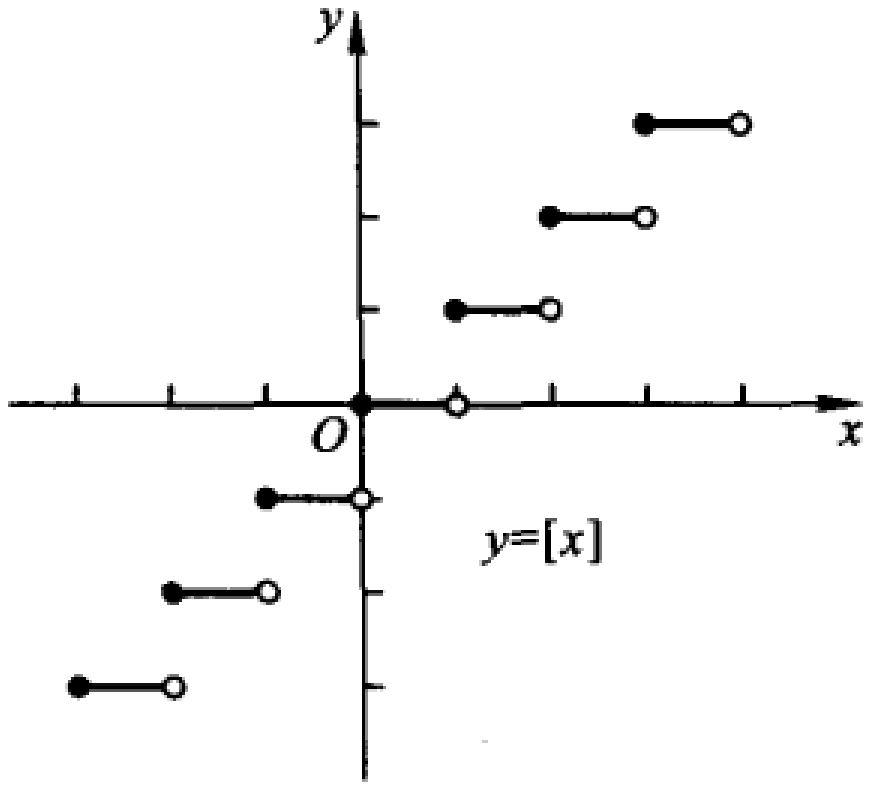
\includegraphics[width=0.72\textwidth]{work/figures/fig2-1}\figcap\label{fig:2-1}
\end{minipage}\hfill
\begin{minipage}[c]{0.48\textwidth}\centering
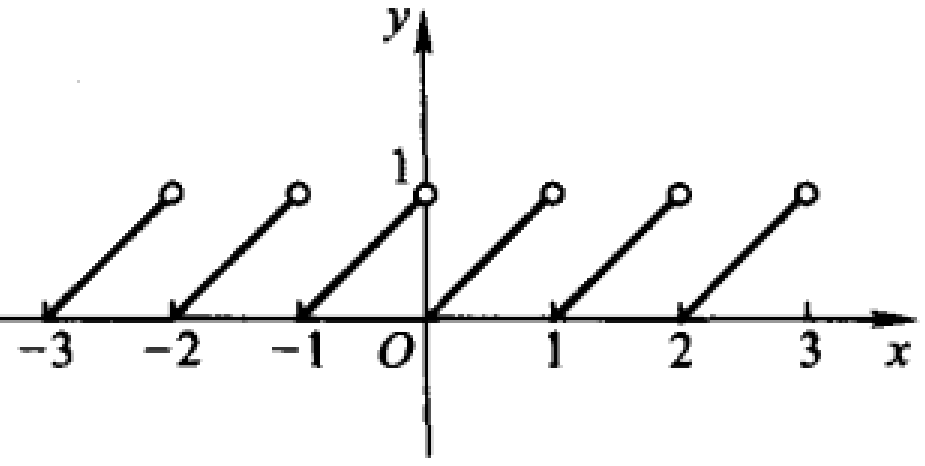
\includegraphics[width=0.72\textwidth]{work/figures/fig2-2}\figcap\label{fig:2-2}
\end{minipage}
\end{figure}

必须指出：函数 $f$ 是一种对应法则，它不是数，符号 $f\colon X\to\mathbb{R}$ 更明显地表示了这一点．然而符号 $y=f(x)$ 对每一个固定的 $x\in X$，它是一个数，是 $f$ 在 $x$ 处取的值．但如果理解 $x$ 可以取遍 $X$，那它也表示一个函数，而且它还有便于计算的优点．因此，以后大多采用这种记号．它既可表示函数，又可表示函数值．

\begin{example}\label{ex:2-1-2}
\[
f(x)=|x|=\begin{cases}
x, & x\geqslant0,\\
-x, & x<0.
\end{cases}
\]
\end{example}

\begin{figure}[htbp]
\centering
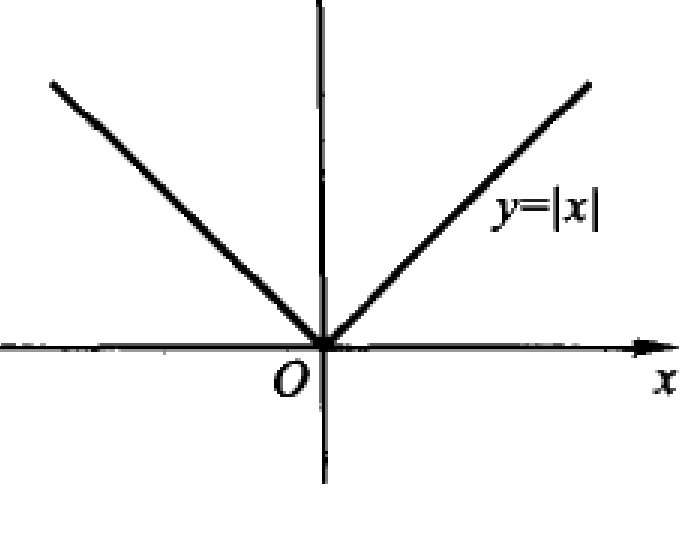
\includegraphics[width=0.36\textwidth]{work/figures/fig2-3}
\figcap\label{fig:2-3}
\end{figure}

这是定义在 $(-\infty,+\infty)$ 上的函数，它在定义域的不同部分分别由不同的表达式给出对应关系．这样定义的函数称为分段函数．注意这不是两个函数，而是一个函数，它给出的是一个对应法则．当 $x\geqslant0$ 时，由表达式 $x$ 确定对应关系；而当 $x<0$ 时，由表达式 $-x$ 确定对应关系．其图形如图~\ref{fig:2-3} 所示．

\begin{example}\label{ex:2-1-3}
\[
D(x)=\begin{cases}
1, & x\text{ 是有理数},\\
0, & x\text{ 是无理数}.
\end{cases}
\]
这个函数称为狄利克雷（Dirichlet，1806---1859）函数．定义域 $X=\mathbb{R}$，值域 $f(X)=\{0,1\}$．此函数的自变量可以认为是连续量，而因变量则显然不是连续量．这个函数在数学史中起过重要作用，它帮助澄清过许多概念．显然这个函数的图形是无法画出来的．
\end{example}

\begin{example}\label{ex:2-1-4}
考虑直线 $y=ax$（$a>0$）与直线 $x=x_0$（$x_0>0$）以及 $x$ 轴所围成的三角形的面积 $s$，有
\[
s(x_0)=\frac{1}{2}ax_0^2.
\]
当 $x_0$ 在 $(0,+\infty)$ 中变动时，我们可以得到函数
\[
s(x)=\frac{1}{2}ax^2,\qquad x>0.
\]
\end{example}

\begin{figure}[htbp]
\centering
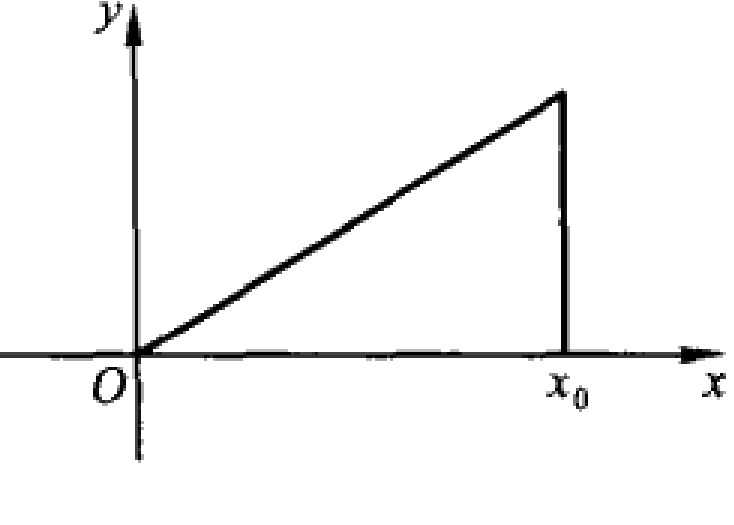
\includegraphics[width=0.38\textwidth]{work/figures/fig2-4}
\figcap\label{fig:2-4}
\end{figure}

这里定义域 $X=(0,+\infty)$ 是实际问题本身所决定的．而就表达式 $\frac{1}{2}ax^2$ 来说，对每一 $x\in(-\infty,+\infty)$，都可确定唯一的值．因此
\[
s(x)=\frac{1}{2}ax^2,\qquad x\in(-\infty,+\infty)
\]
也是一函数．$(-\infty,+\infty)$ 称为 $s(x)$ 的自然定义域，即使得该表达式有意义的所有 $x$ 构成的集合．以后写出一个函数表达式，如没有特别说明，自然就认为它的定义域是它的自然定义域．

\begin{example}\label{ex:2-1-5}
$y=\sqrt{\sin x}$．它表示一个函数，其定义域为 $2k\pi\leqslant x\leqslant (2k+1)\pi$，$k=0,\pm1,\pm2,\cdots$．
\end{example}

\begin{example}\label{ex:2-1-6}
常值函数 $f(x)=c$，$x\in X$．这是一个特殊的函数，对定义域内任一点，其函数值均为常数 $c$．
\end{example}

下面讨论函数的几种特性．

\subsection*{一、函数的奇偶性}

\begin{definition}\label{def:2-2}
设 $X$ 是关于原点对称的（即若 $x\in X$，则 $-x\in X$），$f$ 是定义在 $X$ 上的函数．若对任意 $x\in X$，有 $f(x)=-f(-x)$，则称 $f(x)$ 为奇函数；若对任意 $x\in X$，有 $f(x)=f(-x)$，则称 $f(x)$ 为偶函数．
\end{definition}

奇函数的图形特点是关于原点对称，而偶函数的图形特点是关于 $y$ 轴对称．例如，$y=x^3$ 是奇函数，而 $y=x^2$ 是偶函数，它们的图形分别如下：

\begin{figure}[htbp]
\centering
\begin{minipage}[c]{0.48\textwidth}\centering
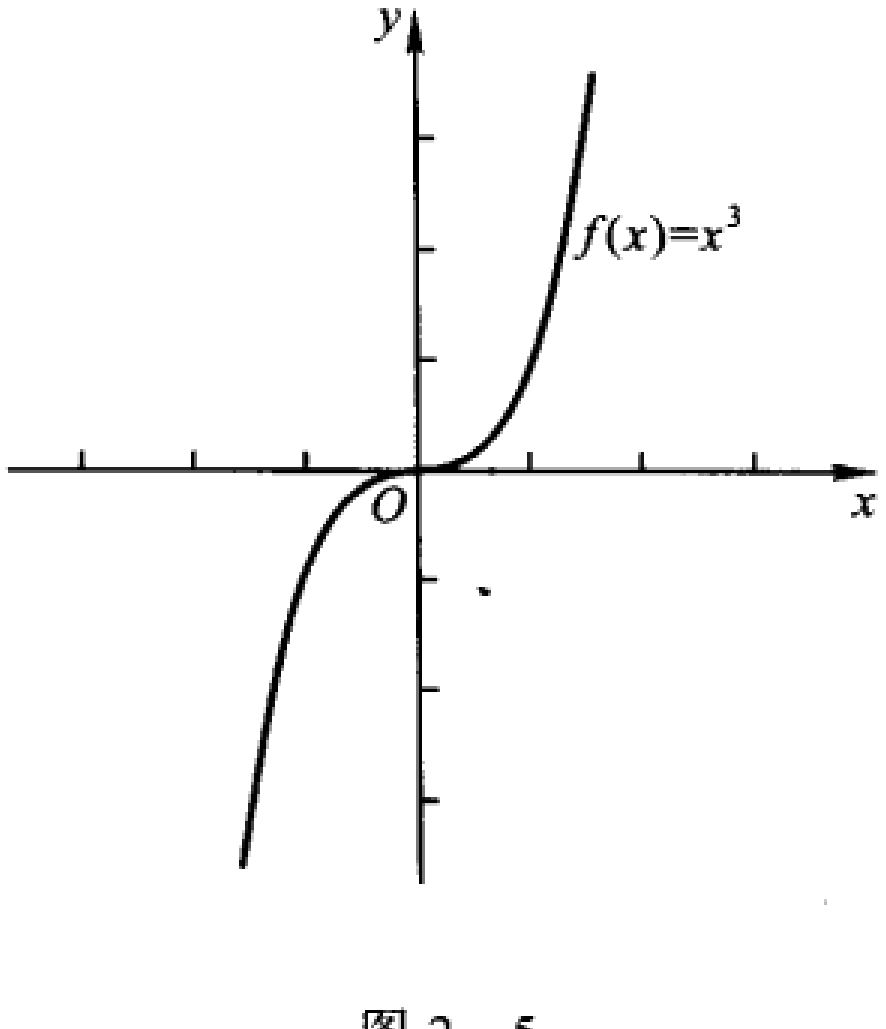
\includegraphics[width=0.72\textwidth]{work/figures/fig2-5}\figcap\label{fig:2-5}
\end{minipage}\hfill
\begin{minipage}[c]{0.48\textwidth}\centering
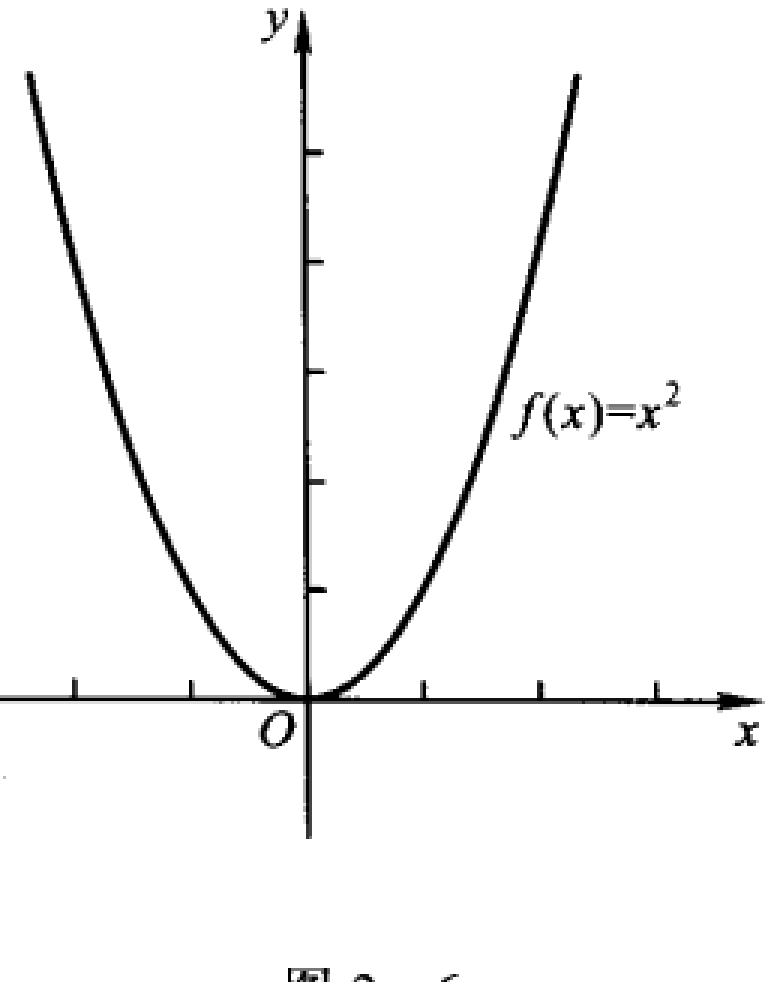
\includegraphics[width=0.72\textwidth]{work/figures/fig2-6}\figcap\label{fig:2-6}
\end{minipage}
\end{figure}

\subsection*{二、函数的单调性}

\begin{definition}\label{def:2-3}
设 $f(x)$ 是定义在 $X$ 上的函数．若对任意 $x_1,x_2\in X$，$x_1<x_2$，有 $f(x_1)\leqslant f(x_2)$，则称 $f(x)$ 在 $X$ 上单调上升或单调递增；若对任意 $x_1,x_2\in X$，$x_1<x_2$，有 $f(x_1)\geqslant f(x_2)$，则称 $f(x)$ 在 $X$ 上单调下降或单调递减．

当上述各不等号为严格不等时，分别称为严格单调上升和严格单调下降．单调上升和单调下降函数统称为单调函数．
\end{definition}

例如 $y=x^3$ 在 $(-\infty,+\infty)$ 是严格单调上升的；$y=x^2$ 在 $(-\infty,0)$ 严格单调下降，而在 $(0,+\infty)$ 是严格单调上升的，但在 $(-\infty,+\infty)$ 不是单调的．又 $y=[x]$ 在 $(-\infty,+\infty)$ 是单调上升，但非严格单调上升．

\subsection*{三、函数的周期性}

\begin{definition}\label{def:2-4}
设函数 $f(x)$ 在 $X$ 上有定义．若存在正数 $T>0$，对任意 $x\in X$，有 $x+T\in X$，且 $f(x+T)=f(x)$，则称 $f(x)$ 是周期函数，$T$ 称为 $f(x)$ 的周期．
\end{definition}

显然，若 $T$ 是 $f(x)$ 的周期，则 $2T,3T,\cdots$ 都是 $f(x)$ 的周期．通常函数的周期是指它的最小周期（如果存在的话）．

例如，$y=\sin x$ 的周期是 $2\pi$；$y=|\sin x|$ 的周期为 $\pi$．但并不是所有周期函数都有最小周期．例如，狄利克雷函数
\[
D(x)=\begin{cases}
1, & x\text{ 是有理数},\\
0, & x\text{ 是无理数}.
\end{cases}
\]
因为任意正有理数都是它的周期，而正有理数是没有最小（正有理）数的．

周期函数的图形可将一个周期上的图形逐段平移而得到．也就是说只要知道了函数在一个周期上的图形，便可作出整个函数的图形．

\subsection*{四、函数的有界性}

\begin{definition}\label{def:2-5}
设 $f(x)$ 在 $X$ 上有定义．若存在 $M>0$，对任意 $x\in X$，有
\[
|f(x)|\leqslant M,
\]
则称 $f(x)$ 在 $X$ 上有界．
\end{definition}

注意，上式又等价于
\[
-M\leqslant f(x)\leqslant M,\qquad x\in X.
\]
在几何上，它表示函数 $f(x)$ 的图形完全位于直线 $y=-M$ 和 $y=M$ 之间．例如，$y=x-[x]$ 在 $(-\infty,+\infty)$ 是有界的，因为存在 $M=1$，使得
\[
|x-[x]|\leqslant 1,\qquad x\in(-\infty,+\infty).
\]
事实上从函数的图形明显可知，$0\leqslant x-[x]<1$（参见图~\ref{fig:2-2}）．

\begin{proposition}\label{prop:2-1}
$f(x)$ 在 $X$ 上有界的充要条件是存在 $A,B$，使得
\[
A\leqslant f(x)\leqslant B,\qquad x\in X.
\]
\end{proposition}

\begin{proof}
必要性：已知 $f(x)$ 有界，即
\[
|f(x)|\leqslant M,\qquad x\in X,
\]
它等价于
\[
-M\leqslant f(x)\leqslant M,\qquad x\in X.
\]
取 $A=-M$，$B=M$，必要性获证．

充分性：已知
\[
A\leqslant f(x)\leqslant B,\qquad x\in X,
\]
取 $M=\max(|A|,|B|)$，则
\[
\begin{aligned}
f(x) &\leqslant B\leqslant |B|\leqslant M,\\
-f(x) &\leqslant -A\leqslant |A|\leqslant M,
\end{aligned}
\]
即
\[
|f(x)|\leqslant M,\qquad x\in X.
\]
充分性获证，从而命题证完．
\end{proof}

这个命题很简单，但即使是这样简单的命题的证明，我们也要求读者能把它写清楚．

通常称命题中的 $A$ 为 $f(x)$ 在 $X$ 上的下界，称 $B$ 为 $f(x)$ 在 $X$ 上的上界．命题~\ref{prop:2-1} 说的是，$f(x)$ 在 $X$ 有界的充要条件是它有上界且有下界．

$f(x)$ 在 $X$ 上无界与 $f(x)$ 在 $X$ 上有界是互相排斥的，两者必居其一．因此，$f(x)$ 在 $X$ 上无界，即是说不存在 $M>0$，使得对所有的 $x\in X$，都满足 $|f(x)|\leqslant M$．但是这样的说法不易验证，为此，我们从正面来叙述，或用肯定的语气来叙述为：对任意 $M>0$，都存在 $x_0\in X$，使得 $|f(x_0)|>M$．

\begin{example}\label{ex:2-1-7}
证明 $f(x)=\frac{1}{x}$ 在 $(0,1)$ 内无界．
\end{example}

\begin{proof}
对任意 $M>0$，取 $x_0=\frac{1}{M+1}\in(0,1)$，则
\[
|f(x_0)|=f(x_0)=\frac{1}{x_0}=M+1>M.
\]
故 $f(x)=\frac{1}{x}$ 在 $(0,1)$ 内无界．
\end{proof}

读者不妨考虑一下，如果不用无界的这种“肯定语气”，这个题目怎样做？

\begin{xiti}
\item 证明下列不等式：
  \begin{ziti}
  \item $|x-y|\geqslant\bigl||x|-|y|\bigr|$；
  \item $|x_1+x_2+\cdots+x_n|\leqslant|x_1|+|x_2|+\cdots+|x_n|$；
  \item $|x_1+x_2+\cdots+x_n+x|\geqslant|x|-(|x_1|+|x_2|+\cdots+|x_n|)$．
  \end{ziti}
\item 求证 $\dfrac{|a+b|}{1+|a+b|}\leqslant\dfrac{|a|}{1+|a|}+\dfrac{|b|}{1+|b|}$．
\item 求证
\[
\max(a,b)=\frac{a+b}{2}+\frac{|a-b|}{2};\qquad \min(a,b)=\frac{a+b}{2}-\frac{|a-b|}{2}.
\]
\item 已知三角形的两条边分别为 $a$ 和 $b$，它们之间的夹角为 $\theta$，试求此三角形的面积 $s(\theta)$，并求其定义域．
\item 在半径为 $r$ 的球内嵌入一内接圆柱，试将圆柱的体积表为其高的函数，并求此函数的定义域．
\item 某公共汽车路线全长为 $20\,\mathrm{km}$，票价规定如下：乘坐 $5\,\mathrm{km}$ 以下（包括 $5\,\mathrm{km}$）者收费 $1$ 元；超过 $5\,\mathrm{km}$ 但在 $15\,\mathrm{km}$ 以下（包括 $15\,\mathrm{km}$）者收费 $2$ 元；其余收费 $2$ 元 $5$ 角．试将票价表为路程的函数，并作出函数的图形．
\item 一脉冲发生器产生一个三角波．若记它随时间 $t$ 的变化规律为 $f(t)$，且三个角分别有对应关系 $f(0)=0$，$f(10)=20$，$f(20)=0$，求 $f(t)$（$0\leqslant t\leqslant 20$），并作出函数的图形．
\item 判别下列函数的奇偶性：
  \begin{ziti}
  \item $f(x)=\dfrac{x^4}{2}+x^2-1$；
  \item $f(x)=x+\sin x$；
  \item $f(x)=x^2\mathrm{e}^{-x^2}$；
  \item $f(x)=\lg(x+\sqrt{1+x^2})$．
  \end{ziti}
\item 判别下列函数是否是周期函数，若是，试求其周期：
  \begin{ziti}
  \item $f(x)=\cos x^2$；
  \item $f(x)=\cos\dfrac{x}{2}+2\sin\dfrac{x}{3}$；
  \item $f(x)=\cos\dfrac{\pi}{4}x$；
  \item $f(x)=\sqrt{\tan x}$．
  \end{ziti}
\item 证明 $f(x)=\dfrac{x}{x^2+1}$ 在 $(-\infty,+\infty)$ 有界．
\item 用肯定语气叙述函数 $f(x)$ 在 $(a,b)$ 无界，并证明 $f(x)=\dfrac{1}{x^2}$ 在 $(0,1)$ 无界．
\item 试证两个偶函数的乘积是偶函数，两个奇函数的乘积是偶函数，一个奇函数与一个偶函数的乘积是奇函数．
\item 设 $f(x)$ 为定义在 $(-\infty,+\infty)$ 内的任何函数，证明 $f(x)$ 可分解成奇函数与偶函数之和．
\item 用肯定语气叙述：在 $(-\infty,+\infty)$ 上
  \begin{ziti}
  \item $f(x)$ 不是奇函数；
  \item $f(x)$ 不是单调上升函数；
  \item $f(x)$ 无零点；
  \item $f(x)$ 无上界．
  \end{ziti}
\end{xiti}

\section{复合函数与反函数}\label{sec:2.2}

有了函数的概念后，我们来讨论函数的运算，这样就可以从几个最简单的函数出发，通过运算来获得更多、更复杂的函数．函数的加、减、乘、除四则运算是大家已经熟知的了，本节主要讨论函数的复合运算和取反函数运算．

\subsection*{1. 复合函数}

我们已经知道自由落体运动中，速度 $v$ 与时间 $t$ 的关系是
\[
v=gt,
\]
而质点的动能为 $M=\frac{1}{2}mv^2$，这样动能依赖于时间的变化关系为
\[
M=\frac{1}{2}mv^2,\qquad v=gt,
\]
或
\[
M=\frac{1}{2}mg^2t^2.
\]
可见 $v$ 在这里起的是桥梁作用．我们称它为中间变量，通过中间变量架起的桥梁，将两个函数复合为一个函数．

\begin{definition}\label{def:2-6}
设函数 $y=f(u)$ 的定义域为 $U$，$u=g(x)$ 的定义域为 $X$，且 $g(X)\subset U$，则 $y=f(g(x))$ 是定义在 $X$ 上的函数，称为 $f$ 与 $g$ 的复合函数，有时也记为 $f\circ g$．$u$ 称为中间变量．
\end{definition}

定义中条件 $g(X)\subset U$ 保证了 $f\circ g$ 确实能给出一个对应法则．这时对每一个 $x\in X$，都有 $g(x)\in U$．而 $f$ 是定义在 $U$ 上的函数，因而有唯一的 $y$ 与 $g(x)$ 对应，也就是说有唯一的 $y$ 与 $x$ 对应．这样就建立了 $X$ 上的对应法则 $f\circ g$．更一般地，若 $g(X)\cap U\neq\emptyset$，仍可得到复合函数 $f\circ g$，但这时复合函数的定义域不是 $X$，而是 $X$ 的一个子集 $X_1=\{x\in X\mid g(x)\in U\}$．可见并不是任意两个函数都可进行复合而成为复合函数，关键在于它们的复合是否确能给出一个对应法则．例如，$u=g(x)=1+a^x$，$y=f(u)=\sqrt{1-u^2}$，显然函数 $f$ 的定义域为 $[-1,1]$，而 $g(x)>1$，因此不可能通过 $u$ 复合为函数．

\begin{example}\label{ex:2-2-1}
设
\[
f(x)=\begin{cases}
x+1, & x>1,\\
x^2, & x\leqslant1,
\end{cases}\qquad g(x)=5x+3.
\]
求 $f(g(x))$ 和 $g(f(x))$．
\end{example}

\begin{proof}[解]
$f(x)$ 和 $g(x)$ 的定义域都是 $(-\infty,+\infty)$，所以存在复合函数 $f(g(x))$ 和 $g(f(x))$．又 $5x+3>1$ 当且仅当 $x>-\frac{2}{5}$，故有
\[
f(g(x))=\begin{cases}
5x+4, & x>-\frac{2}{5},\\
(5x+3)^2, & x\leqslant-\frac{2}{5},
\end{cases}
\]
\[
g(f(x))=\begin{cases}
5(x+1)+3, & x>1,\\
5x^2+3, & x\leqslant1.
\end{cases}
\]
\end{proof}

从上述例子可见，一般说来，复合运算并不满足交换律，即 $f\circ g\neq g\circ f$．

\subsection*{2. 反函数}

在匀速直线运动中，有关系式 $s=vt$，这里时间 $t$ 是自变量，路程 $s$ 是因变量，由时间可计算出路程．但也会出现这样的情形，即已测得路程 $s$，要求推算时间 $t$，也就是说要求把 $s$ 作为自变量，$t$ 作为因变量．可见自变量与因变量往往是相对的．那么什么情况下可以使自变量与因变量相互转化呢？这就是反函数的概念．

\begin{definition}\label{def:2-7}
设 $y=f(x)$ 是定义在 $X$ 上的函数．如果对值域 $f(X)$ 的每个 $y$，都有唯一的 $x\in X$，使得 $f(x)=y$，则这样定义的 $x$ 作为 $y$ 的函数，称为 $f$ 的反函数，记为 $f^{-1}$，即
\[
f^{-1}\colon y\to x,\qquad \text{如果 } y=f(x).
\]
\end{definition}

并不是所有的函数都有反函数存在．例如，$y=x^2$，$x\in(-\infty,+\infty)$．对每个 $y>0$，与之对应的 $x$ 不唯一，因为有两个值 $x=\pm\sqrt{y}$ 满足 $y=x^2$，因此不能确定从 $(0,+\infty)$ 到 $\mathbb{R}$ 的对应关系．很容易看出，反函数存在的条件是：对任意 $x_1,x_2\in X$，$x_1\neq x_2$，有 $f(x_1)\neq f(x_2)$．也就是说，$f$ 在 $X$ 与 $f(X)$ 之间建立的是一个一一对应的关系．由此得到，若 $f(x)$ 在 $X$ 严格单调，则它一定有反函数存在．显然，如果函数 $f$ 有反函数 $f^{-1}$ 存在，那么
\[
f^{-1}(f(x))=x,\quad \forall x\in X,
\]
\[
f(f^{-1}(y))=y,\quad \forall y\in f(X),
\]
其中“$\forall$”是逻辑符号，意指“对任意”．

函数与反函数，是对应关系为互逆，用什么字母表示是不重要的，但通常我们习惯于用 $x$ 表示自变量，用 $y$ 表示因变量．因此 $y=f(x)$，$x\in X$ 的反函数仍写为
\[
y=f^{-1}(x),\qquad x\in f(X).
\]
它与
\[
x=f^{-1}(y),\qquad y\in f(X)
\]
是同一函数，因为对应法则都是 $f^{-1}$，定义域也都是 $f$ 的值域 $f(X)$．

\begin{example}\label{ex:2-2-2}
函数 $y=x^2$，$x\in(0,+\infty)$ 的反函数为
\[
x=\sqrt{y},\qquad y\in(0,+\infty),
\]
或
\[
y=\sqrt{x},\qquad x\in(0,+\infty).
\]
其图形如图~\ref{fig:2-7} 所示．
\end{example}

\begin{figure}[htbp]
\centering
\begin{minipage}[c]{0.48\textwidth}\centering
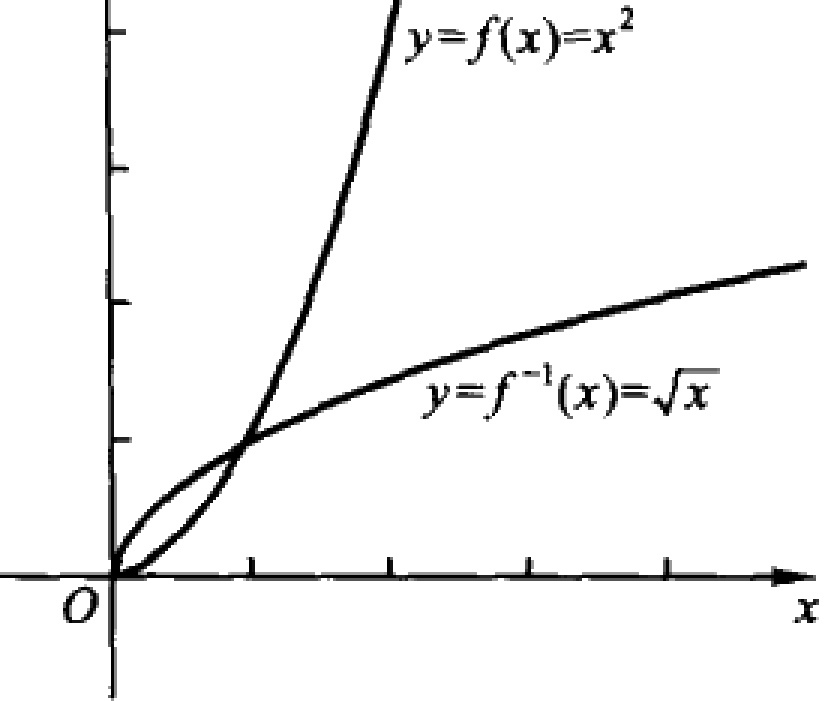
\includegraphics[width=0.72\textwidth]{work/figures/fig2-7}\figcap\label{fig:2-7}
\end{minipage}\hfill
\begin{minipage}[c]{0.48\textwidth}\centering
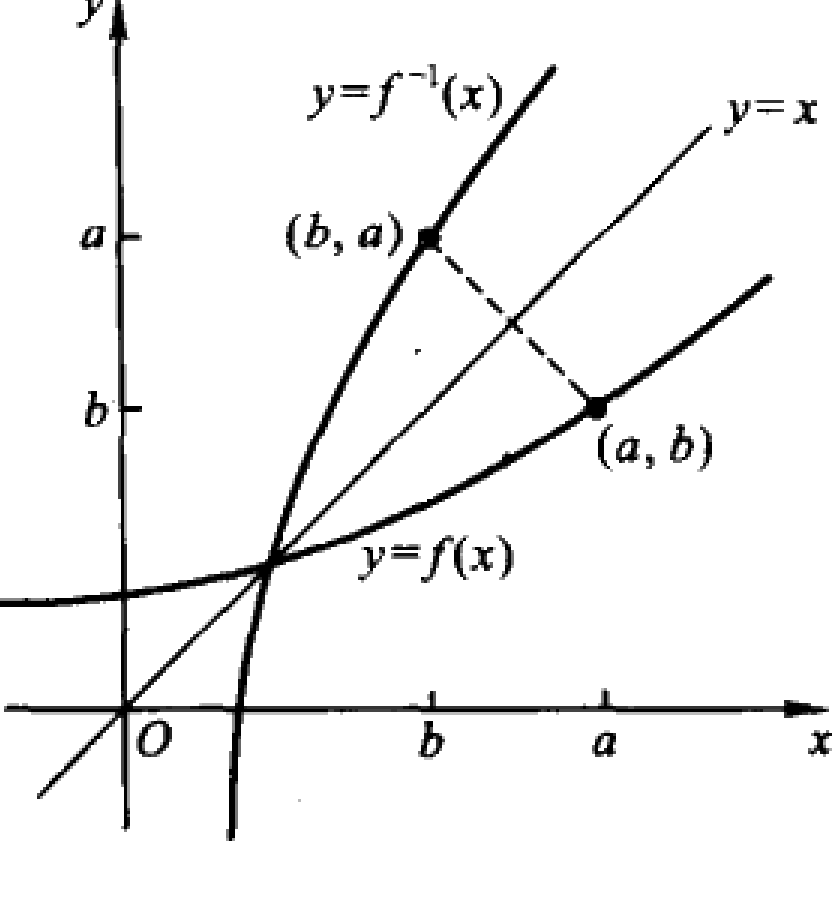
\includegraphics[width=0.72\textwidth]{work/figures/fig2-8}\figcap\label{fig:2-8}
\end{minipage}
\end{figure}

在作函数的图形时，我们也往往习惯于用横坐标表示自变量，用纵坐标表示因变量．这时 $y=f^{-1}(x)$ 的图形与 $y=f(x)$ 的图形有什么关系呢？若 $(a,b)$ 在曲线 $y=f(x)$ 上，由反函数的定义知，$(b,a)$ 必在曲线 $y=f^{-1}(x)$ 上．而 $(b,a)$ 与 $(a,b)$ 是关于直线 $y=x$ 对称的点．因此 $y=f^{-1}(x)$ 的图形与 $y=f(x)$ 的图形是关于直线 $y=x$ 对称的（见图~\ref{fig:2-8}）．这样，由 $y=f(x)$ 的图形便很容易作出 $y=f^{-1}(x)$ 的图形．

\begin{proposition}\label{prop:2-2}
严格递增（减）的函数必有反函数，且其反函数也是严格递增（减）的．
\end{proposition}

\begin{proof}
反函数存在性是显然的（前面已说过）．设 $f(x)$ 在 $X$ 严格递增，要证 $f^{-1}(y)$ 在 $f(X)$ 也是严格递增的．用反证法．如果不然，存在 $y_1,y_2\in f(X)$，$y_1<y_2$，但 $f^{-1}(y_1)\geqslant f^{-1}(y_2)$，这时 $f(f^{-1}(y_1))\geqslant f(f^{-1}(y_2))$，即 $y_1\geqslant y_2$，矛盾．命题~\ref{prop:2-2} 证完．
\end{proof}

\begin{xiti}
\item 设 $f(x)=\dfrac{1-x}{1+x}$，求证 $f(f(x))=x$．
\item 求下列函数的反函数及其定义域：
  \begin{ziti}
  \item $y=\dfrac{1}{2}\left(x+\dfrac{1}{x}\right)$,\quad $1<x<+\infty$；
  \item $y=\dfrac{1}{2}(\mathrm{e}^x-\mathrm{e}^{-x})$,\quad $-\infty<x<+\infty$；
  \item $y=\begin{cases}
  x, & -\infty<x<1,\\
  x^2, & 1\leqslant x\leqslant 4,\\
  2^x, & 4<x<+\infty.
  \end{cases}$
  \end{ziti}
\item 设 $f(x)$，$g(x)$ 为实轴上单调函数，求证 $f(g(x))$ 也是实轴上的单调函数．
\item 设
\[
f(x)=\begin{cases}
-x-1, & x\leqslant0,\\
x, & x>0,
\end{cases}\qquad g(x)=\begin{cases}
x, & x\leqslant0,\\
-x^2, & x>0.
\end{cases}
\]
求复合函数 $f(g(x)), g(f(x))$．
\item 设 $f(x)=\dfrac{x}{\sqrt{1+x^2}}$，求 $(f\underbrace{\circ f\circ\cdots\circ f}_{n\text{ 次}})(x)$．
\item 设 $f(x)=|1+x|-|1-x|$，试求 $(f\underbrace{\circ f\circ\cdots\circ f}_{n\text{ 次}})(x)$．
\item 设 $f(x)=\dfrac{1}{1-x}$，求 $f(f(x))$，$f(f(f(x)))$，$f\left(\dfrac{1}{f(x)}\right)$．
\end{xiti}

\section{初等函数}\label{sec:2.3}

有了函数的四则运算和复合运算，我们可以从六种函数出发，通过运算来获得更多的函数，这六种函数是常值函数，指数函数，幂函数，对数函数，三角函数和反三角函数．称它们为基本初等函数．

函数若是由基本初等函数经有限次的四则运算和复合所得到，则称为初等函数．否则，称为非初等函数．因此，首先必须熟悉基本初等函数的性质及其图形．

\subsection*{(1) 常值函数}
\[
y=c,\qquad x\in(-\infty,+\infty)
\]
在本章§\ref{sec:2.1}例~\ref{ex:2-1-6}已介绍过．

\subsection*{(2) 指数函数}
\[
y=a^x,\qquad x\in(-\infty,+\infty)\quad(a>0,a\neq1).
\]
函数的值域是 $(0,+\infty)$，图形总经过点 $(0,1)$．当 $a>1$ 时，函数严格单调上升；当 $0<a<1$ 时，函数严格单调下降．$a^x$ 与 $\left(\frac{1}{a}\right)^x$ 的图形关于 $y$ 轴对称（见图~\ref{fig:2-9}）．

\subsection*{(3) 对数函数}
\[
y=\log_a x,\qquad x\in(0,+\infty)\quad(a>0,a\neq1).
\]
对数函数与指数函数互为反函数．因此由指数函数的性质立即知，对数函数的值域是 $(-\infty,+\infty)$，图形总经过点 $(1,0)$，当 $a>1$ 时，函数严格单调上升；当 $0<a<1$ 时，函数严格单调下降．$\log_a x$ 与 $\log_{\frac{1}{a}}x$ 的图形关于 $x$ 轴对称（见图~\ref{fig:2-10}）．

\begin{figure}[htbp]
\centering
\begin{minipage}[c]{0.48\textwidth}\centering
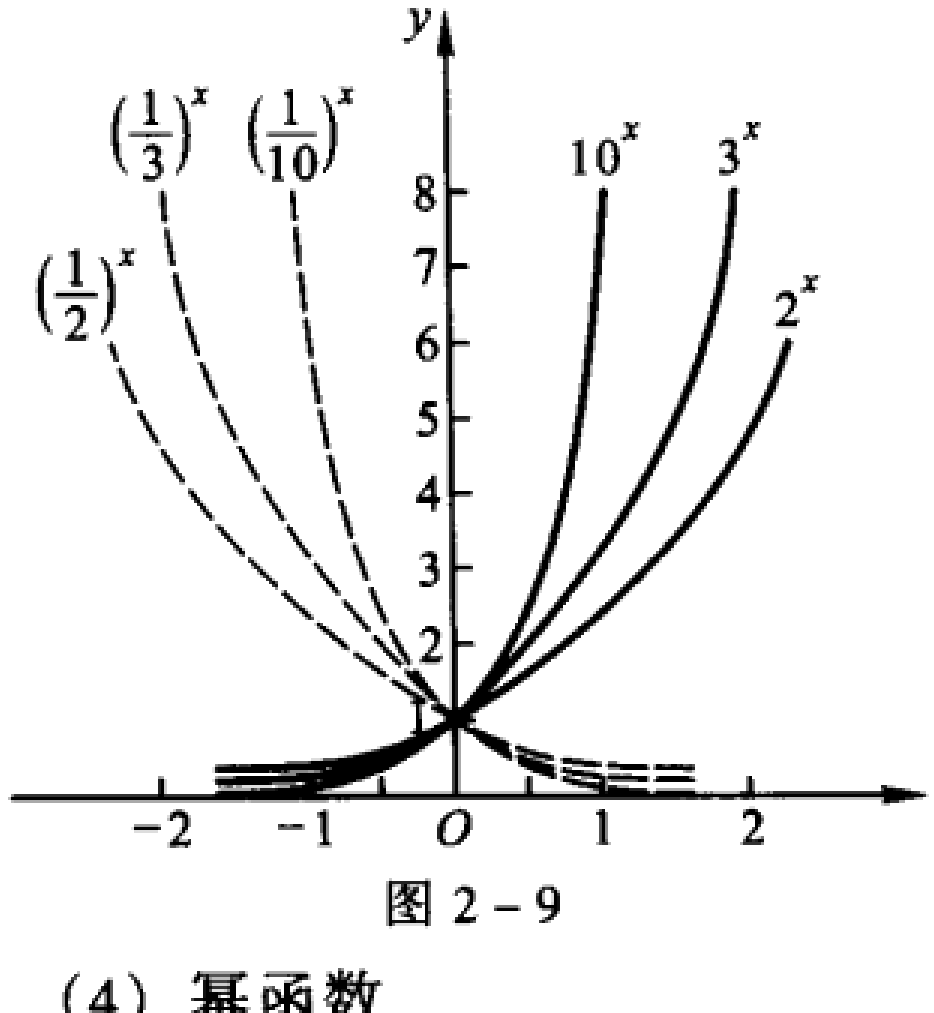
\includegraphics[width=0.72\textwidth]{work/figures/fig2-9}\figcap\label{fig:2-9}
\end{minipage}\hfill
\begin{minipage}[c]{0.48\textwidth}\centering
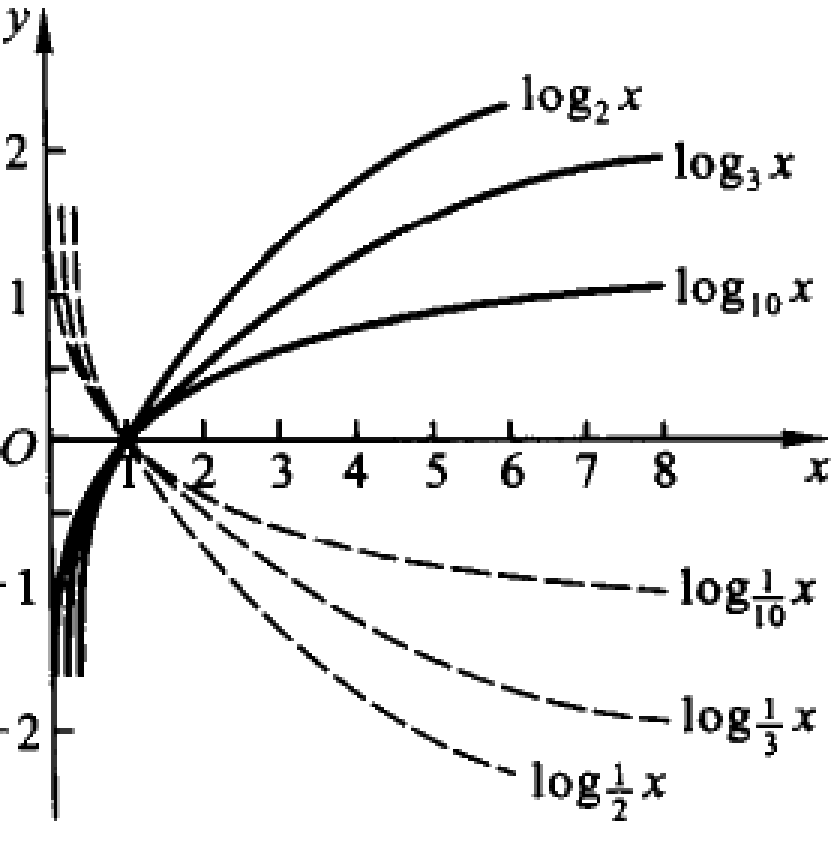
\includegraphics[width=0.72\textwidth]{work/figures/fig2-10}\figcap\label{fig:2-10}
\end{minipage}
\end{figure}

\subsection*{(4) 幂函数}
\[
y=x^{\mu},\qquad \text{其中 }\mu\neq0.
\]
幂函数的定义域根据 $\mu$ 值的不同而不同．当 $\mu=\frac{p}{q}$ 是有理数时（其中 $p,q$ 是整数，且 $p,q$ 互素），其定义域见下表：

\begin{table}[htbp]
\centering
\begin{tabular}{|c|c|c|}
\hline
\multicolumn{2}{|c|}{$\mu = \frac{p}{q}$} & 定义域 \\
\hline
\multirow{2}{*}{$\mu > 0$} & $q$ 为奇数 & $(-\infty, +\infty)$ \\
\cline{2-3}
 & $q$ 为偶数 & $[0, +\infty)$ \\
\hline
\multirow{2}{*}{$\mu < 0$} & $q$ 为奇数 & $(-\infty, 0) \cup (0, +\infty)$ \\
\cline{2-3}
 & $q$ 为偶数 & $(0, +\infty)$ \\
\hline
\end{tabular}
\end{table}

当 $\mu$ 是无理数时，$x^{\mu}$ 定义为 $x^{\mu}=10^{\mu\lg x}$，故定义域为 $(0,+\infty)$．可见不论 $\mu\,(\neq0)$ 为何值，幂函数 $x^{\mu}$ 在 $(0,+\infty)$ 总有定义．

当 $x>0$ 时，$x^{\mu}>0$，故此时函数的图形在第一象限，函数的图形总经过点 $(1,1)$，当 $\mu>0$ 时，函数严格单调上升；当 $\mu<0$ 时，函数严格单调下降．函数 $x^{\mu}$ 和 $x^{\frac{1}{\mu}}$ 互为反函数，图形关于直线 $y=x$ 对称（见图~\ref{fig:2-11} 和图~\ref{fig:2-12}）．

\begin{figure}[htbp]
\centering
\begin{minipage}[c]{0.48\textwidth}\centering
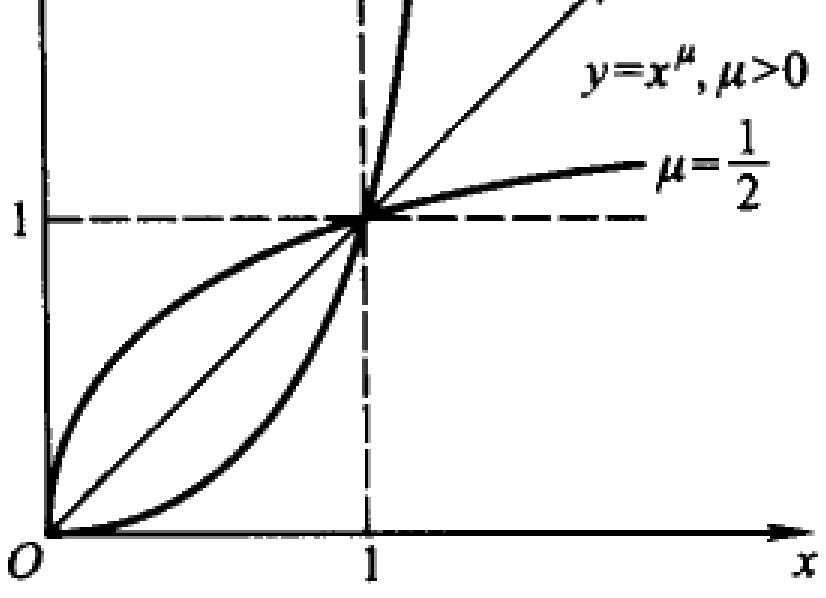
\includegraphics[width=0.72\textwidth]{work/figures/fig2-11}\figcap\label{fig:2-11}
\end{minipage}\hfill
\begin{minipage}[c]{0.48\textwidth}\centering
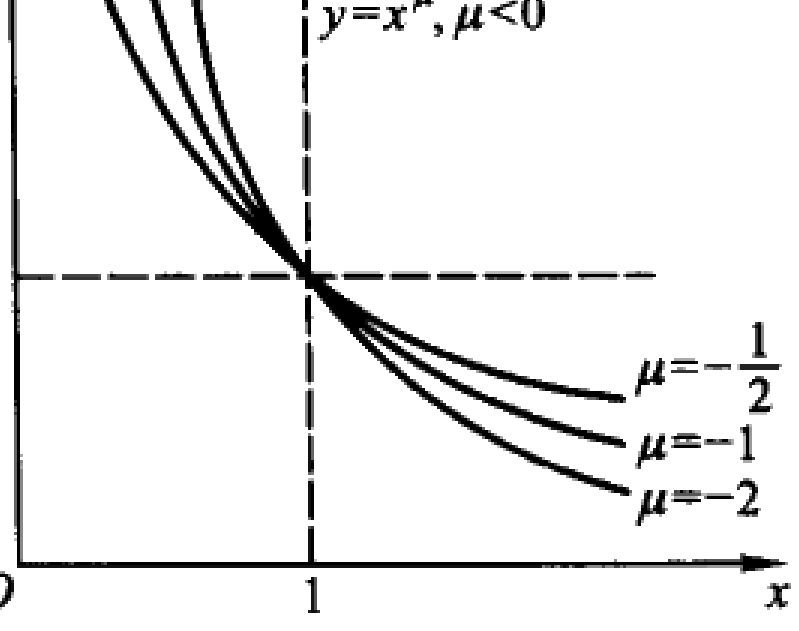
\includegraphics[width=0.72\textwidth]{work/figures/fig2-12}\figcap\label{fig:2-12}
\end{minipage}
\end{figure}

\subsection*{(5) 三角函数}

正弦函数 $y=\sin x$，$x\in(-\infty,+\infty)$；

余弦函数 $y=\cos x$，$x\in(-\infty,+\infty)$；

正切函数 $y=\tan x$，$x\neq k\pi+\frac{\pi}{2}$，$k=0,\pm1,\pm2,\cdots$；

余切函数 $y=\cot x$，$x\neq k\pi$，$k=0,\pm1,\pm2,\cdots$．

这些函数都是周期函数．正弦和余弦函数的周期为 $2\pi$，值域为 $[-1,1]$．正切和余切函数的周期为 $\pi$，值域为 $(-\infty,+\infty)$，它们的图形如图~\ref{fig:2-13} 和图~\ref{fig:2-14} 所示．

注意，在微积分中，三角函数的自变量 $x$ 一般是用弧度．

\begin{figure}[htbp]
\centering
\begin{minipage}[c]{0.48\textwidth}\centering
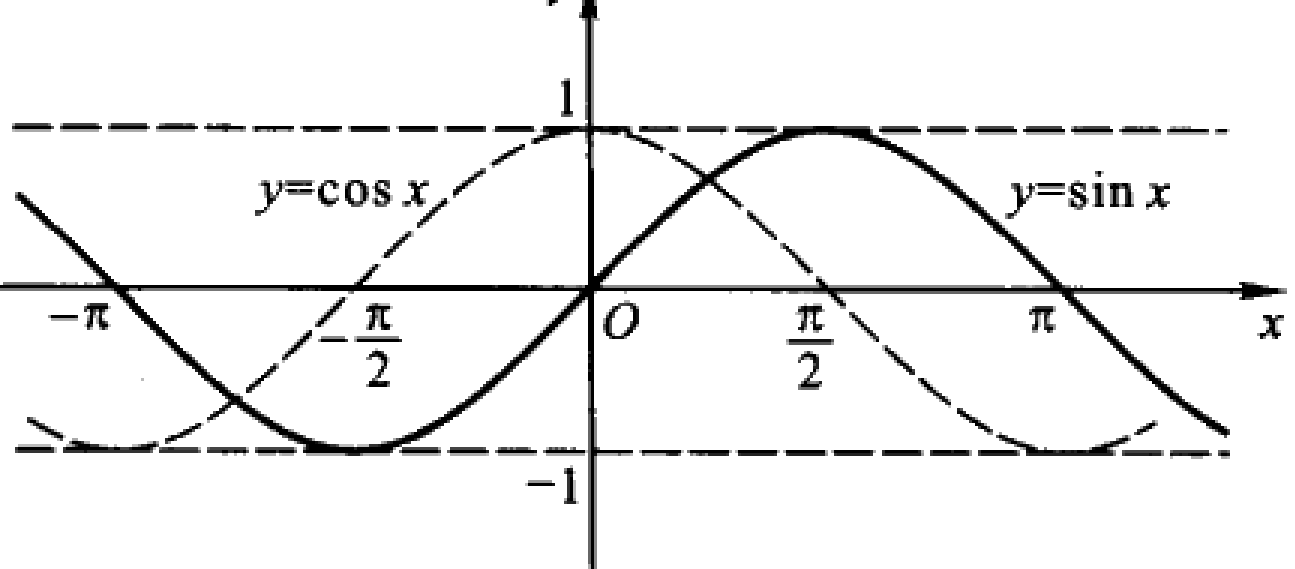
\includegraphics[width=0.78\textwidth]{work/figures/fig2-13}\figcap\label{fig:2-13}
\end{minipage}\hfill
\begin{minipage}[c]{0.48\textwidth}\centering
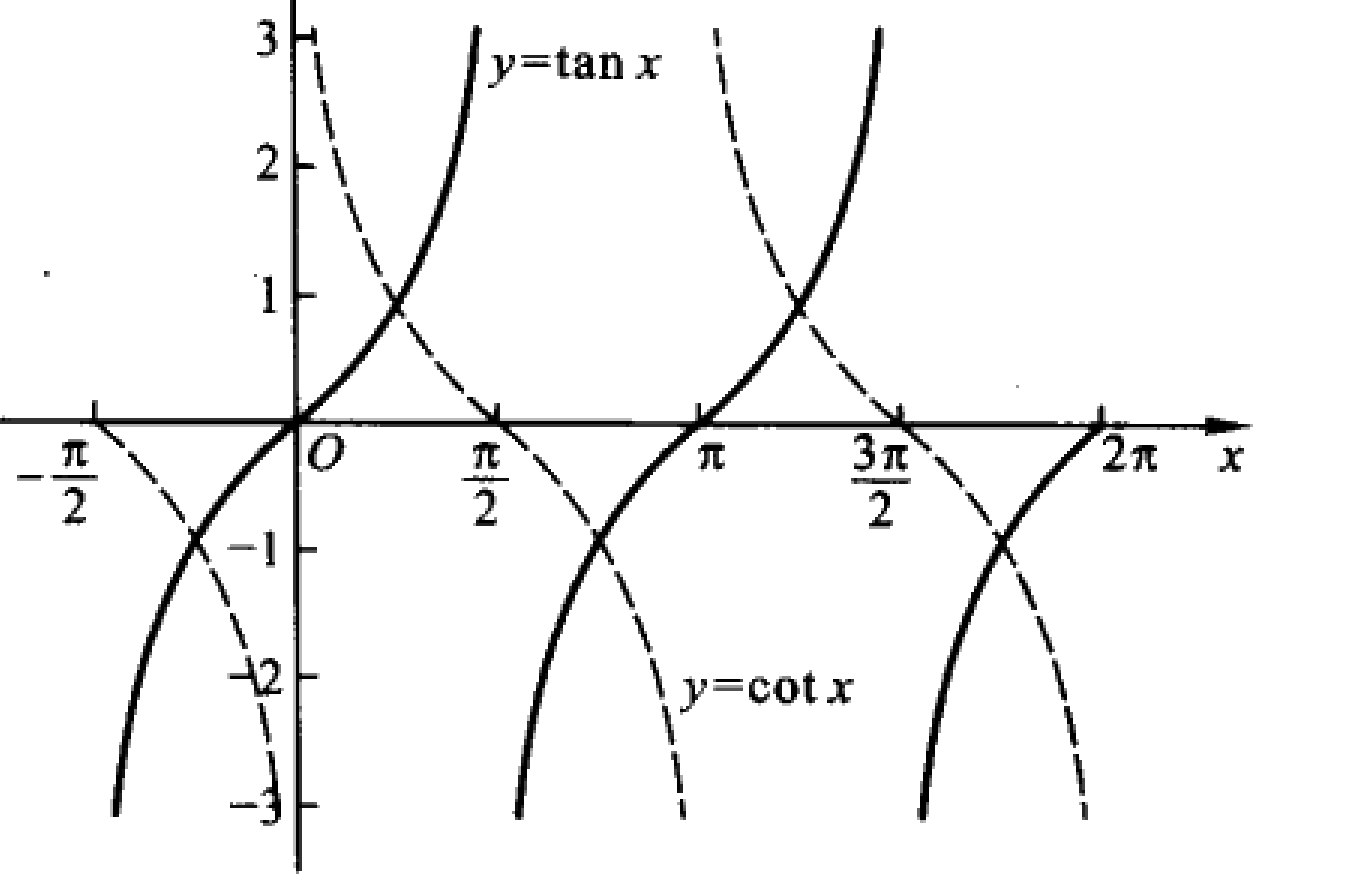
\includegraphics[width=0.78\textwidth]{work/figures/fig2-14}\figcap\label{fig:2-14}
\end{minipage}
\end{figure}

\subsection*{(6) 反三角函数}

因为三角函数不是一一对应的，因此我们只能分别在它们的一个严格单调分支上来讨论反函数．

反正弦函数 $y=\arcsin x$，$x\in[-1,1]$，$y\in\left[-\frac{\pi}{2},\frac{\pi}{2}\right]$；

反余弦函数 $y=\arccos x$，$x\in[-1,1]$，$y\in[0,\pi]$；

反正切函数 $y=\arctan x$，$x\in(-\infty,+\infty)$，$y\in\left(-\frac{\pi}{2},\frac{\pi}{2}\right)$；

反余切函数 $y=\operatorname{arccot} x$，$x\in(-\infty,+\infty)$，$y\in(0,\pi)$．

反正弦和反正切函数在定义域内严格单调上升且是奇函数，而反余弦和反余切函数在定义域内严格单调下降．它们的图形分别见图~\ref{fig:2-15}～图~\ref{fig:2-18}．

\begin{figure}[htbp]
\centering
\begin{minipage}[c]{0.48\textwidth}\centering
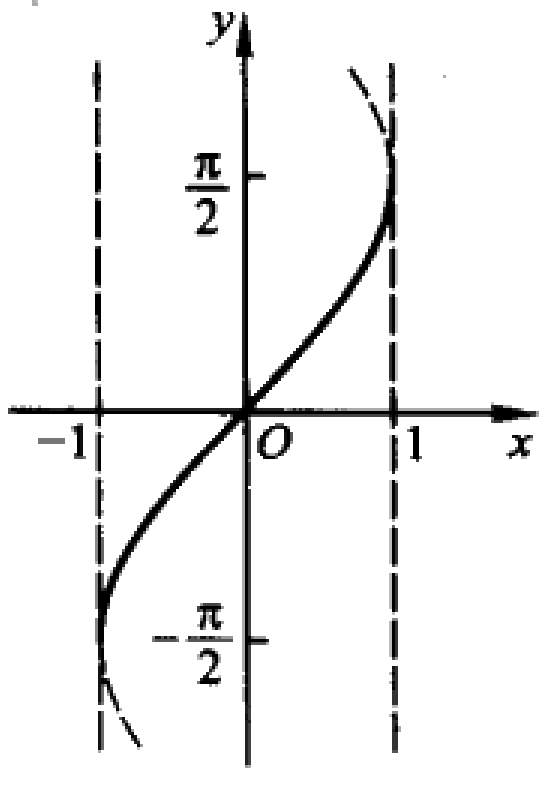
\includegraphics[width=0.70\textwidth]{work/figures/fig2-15}\figcap\label{fig:2-15}
\end{minipage}\hfill
\begin{minipage}[c]{0.48\textwidth}\centering
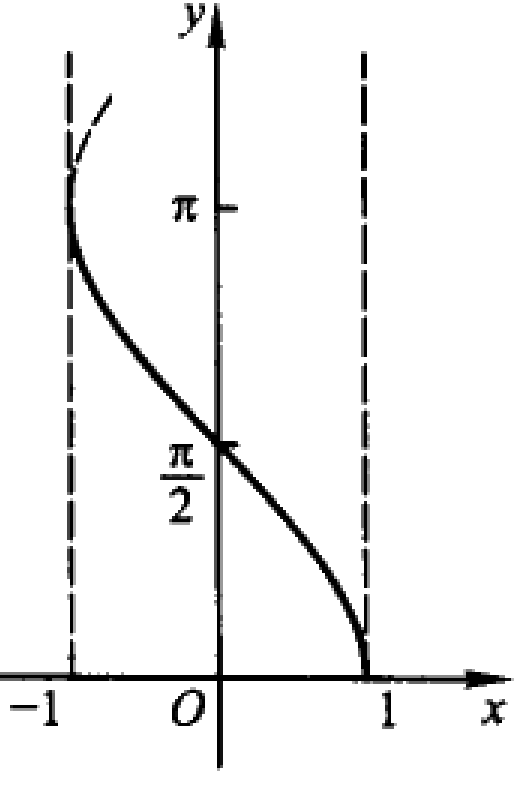
\includegraphics[width=0.70\textwidth]{work/figures/fig2-16}\figcap\label{fig:2-16}
\end{minipage}\\[1em]
\begin{minipage}[c]{0.48\textwidth}\centering
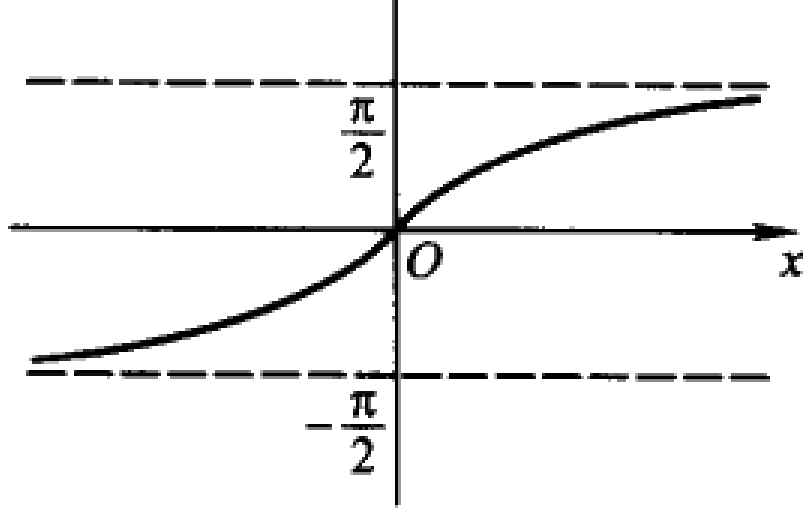
\includegraphics[width=0.70\textwidth]{work/figures/fig2-17}\figcap\label{fig:2-17}
\end{minipage}\hfill
\begin{minipage}[c]{0.48\textwidth}\centering
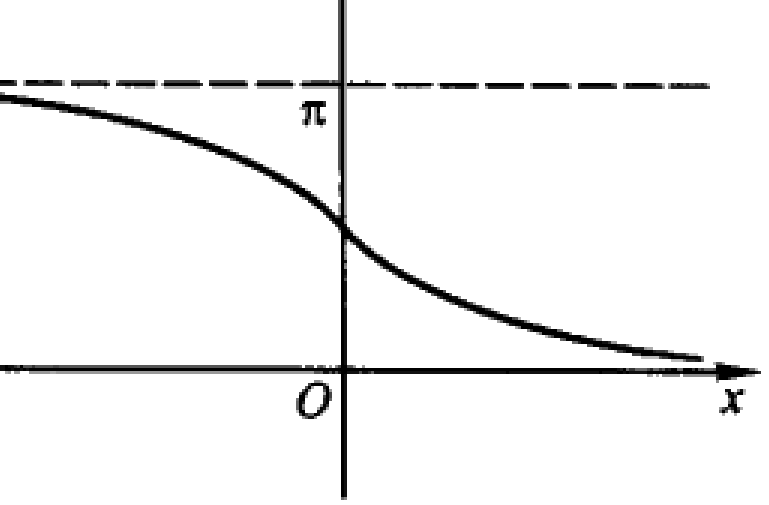
\includegraphics[width=0.70\textwidth]{work/figures/fig2-18}\figcap\label{fig:2-18}
\end{minipage}
\end{figure}

\begin{example}\label{ex:2-3-1}
$y=\arctan 2^{-x}$ 是初等函数，定义域是 $(-\infty,+\infty)$，值域是 $\left(0,\frac{\pi}{2}\right)$．函数在定义域内是严格单调下降的，这是因为 $2^{-x}=\left(\frac{1}{2}\right)^x$ 是严格单调下降的，而 $\arctan x$ 是严格单调上升的．
\end{example}

\begin{example}\label{ex:2-3-2}
作出函数 $y=\sin(2x+\pi)$ 的图形．
\end{example}

\begin{proof}[解]
\[
\sin[2(x+\pi)+\pi]=\sin(2x+\pi)=-\sin 2x,
\]
故函数是以 $\pi$ 为周期的周期函数．先作 $\sin 2x$ 的图形，然后将图形绕 $x$ 轴旋转 $180^\circ$，即得所要作的函数图形（图~\ref{fig:2-19}）．
\end{proof}

\begin{example}\label{ex:2-3-3}
\[
y=\begin{cases}
\mathrm{e}^x, & x\geqslant0,\\
0, & x<0,
\end{cases}
\]
它在每个分段上都是初等函数，但它不是初等函数，这点以后可加以证明．
\end{example}

\begin{figure}[htbp]
\centering
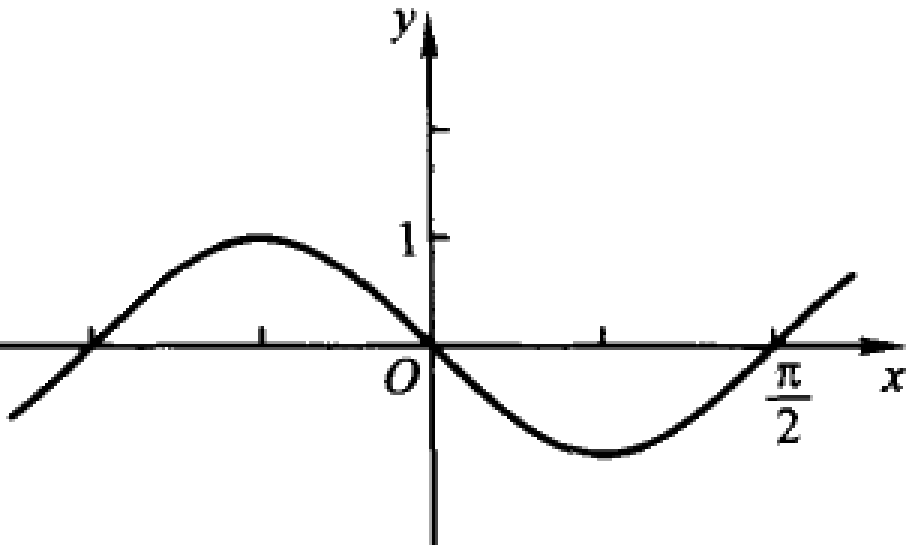
\includegraphics[width=0.48\textwidth]{work/figures/fig2-19}
\figcap\label{fig:2-19}
\end{figure}

\begin{xiti}
\item 对下列函数分别讨论函数的定义域和值域，奇偶性，周期性，有界性，并作出函数的图形：
  \begin{ziti}
  \item $y=|x|$；
  \item $y=x-[x]$；
  \item $y=\tan|x|$；
  \item $y=\sqrt{x(2-x)}$；
  \item $y=\sin^2 x$；
  \item $y=|\sin x|+|\cos x|$．
  \end{ziti}
\item 若已知函数 $y=f(x)$ 的图形，作函数
\[
y_1=|f(x)|,\qquad y_2=f(-x),\qquad y_3=-f(-x)
\]
的图形，并说明 $y_1,y_2,y_3$ 的图形与 $y$ 的图形的关系．
\item 若已知 $f(x),g(x)$ 的图形，试作函数
\[
y=\frac{1}{2}\bigl[f(x)+g(x)\pm\bigl|f(x)-g(x)\bigr|\bigr]
\]
的图形，并说明 $y$ 的图形与 $f(x),g(x)$ 图形的关系．
\item 作出下列函数的图形：
  \begin{ziti}
  \item $y=x\sin x$；
  \item $y=\sin\dfrac{1}{x}$．
  \end{ziti}
\item 符号函数的定义是
\[
y=\sgn x=\begin{cases}
1, & x>0,\\
0, & x=0,\\
-1, & x<0,
\end{cases}
\]
试分别作出 $\sgn x$，$\sgn(2x)$，$\sgn(x-2)$ 的图形．
\item 作出下列函数的图形：
  \begin{ziti}
  \item $y=\sgn\cos x$；
  \item $y=[x]-2\left[\dfrac{x}{2}\right]$．
  \end{ziti}
\end{xiti}
